
%\addcontentsline{toc}{chapter}{Development Process}
\chapter{Design}

%You should concentrate on the more important aspects of the design. It is essential that an overview is presented before going into detail. As well as describing the design adopted it must also explain what other designs were considered and why they were rejected.
\section{Overall Architecture}
\textbf{NOTES: - DELETE THIS -}
\begin{itemize}
\item Tried to make it easy to add new Algorithms or data from different sources. Map-tiles and routing-data stored locally - this is not ideal; compromise to ensure stability. 3rd parties online may take their servers down or make changes to their service. Local copy is always the same - no matter where the system is run.
\item create more sub-sections here? That might look better.
\end{itemize}

The system reads a \textit{.osm} file\cite{OSM-XML} downloaded from OpenStreetMap\cite{OSM}, and separates its contents into two Arrays: Nodes and Ways. This data is then put through a filter to remove any islands (or Nodes/Ways without any connections), in addition to all Nodes/Ways deemed unsuitable for navigation for PRMs.

The \textit{.osm} file also contains information about \textquotedblleft Relations\textquotedblright, but as these represent abstract areas like the outline of a forest or housing-block, they are not useful for pathfinding, and can therefore safely be ignored by the system.\footnote{\textquotedblleft Relations\textquotedblright~also represent things like bus-routes, which could make a route-planner aimed at PRMs even more useful if considered -- but this will be touched on later in this report.}

A Node is a single point on the map -- defined by its Latitude and Longitude coordinates. Nodes can be isolated points of interest like statues or monuments, or they can be part of one or more Ways representing larger structures.

Ways contain an ordered list of Nodes, each of which define its shape, and direction. The ordering of Nodes inside the Way is important in cases where a degree of inclination is indicated, or whenever a route passes through a one-way street.
If the ordering of Nodes is not respected, then a Way's degrees of inclination may get flipped from positive to negative, or a route may become illegal to follow if it goes the wrong way on a one-way street. See Figure \ref{fig:connectionsWays} for an illustration of how Nodes and ways may be represented, and Figure \ref{fig:nodeExpansion} for an illustration of how Ways may be expanded.

Nodes shared between two or more Ways can be thought of as intersections between those Ways. Nodes that are shared between multiple Ways are called \textquotedblleft Tower Nodes\textquotedblright, while unshared Nodes are called \textquotedblleft Pillar Nodes\textquotedblright; See Figure \ref{fig:nodeExpansion}.

Only Tower Nodes are expanded when planning routes, as this speeds up searches, and reduces memory-requirements significantly. Some Ways can contain more than 100 Nodes, but may only have 2-3 Tower Nodes. By ignoring the large majority of a Way's Nodes when planning routes, searches are sped up significantly, and less memory has to be used to keep track of which Nodes were expanded to get to another.

Routes are found by continuously expanding the Nodes connected to other Nodes; starting at a \textquotedblleft Start Node\textquotedblright, and ending at a \textquotedblleft Goal Node\textquotedblright. Some search-algorithms find the shortest path between the two Nodes by using certain heuristics, while others just keep expanding Nodes until the \textquotedblleft Goal Node\textquotedblright~is found, at which point the route is returned -- no matter how good or bad it might be. Both kinds of algorithms will be discussed here, along with their advantages and disadvantages.

All map-tiles and Node/Way data is stored locally. This is because it was too risky to rely on third parties to keep their servers running at all times while the system was being developed. The author's internet-connection was also quite unreliable at times, so making the system rely on online-data would make this project very vulnerable to further delays. Third party mapping-services that were considered but decided against for various reasons: GraphHopper\cite{Graphhopper}, Mapbox\cite{mapbox}, Leaflet\cite{leaflet}, Cloudmade\cite{cloudmade}, Omniscale\cite{omniscale}, OpenLayers\cite{openlayers}, and Google Maps\cite{GoogleMaps}.

\section{Classes and methods}
\textbf{NOTES: - DELETE THIS -}
\begin{itemize}
\item Classes split into separate packages for database-indexing, route-planning, and running the system.
\item Interface for Nodes and Ways? Or are the Node and Way classes the top-level? Double-check.
\item Interface for uninformed search.
\item Interface for Informed search implements interface for uninformed Search.
\item Each search-algorithm inherits all its functionality from those two interfaces - only implements one method: search(or something similar).
\item spiral model%TODO This has not been mentioned yet anywhere in the report
\end{itemize}

Every class has been sorted into one of three packages for database-indexing, route-planning, or running the system. Mapsforge provides the system with many new packages to handle the map, but as these were made by a third party, and accessed via a \textit{.jar}-file, they won't be mentioned here.

The Node- and Way-classes implement an interface to ensure that any new Node/Way classes implemented in the future will still be compatible with the rest of the system, while still allowing them to implement new functionality or store more data.

There is also an interface for \textit{\textquotedblleft Uninformed Search\textquotedblright}, which provides every search-algorithm with the methods they need to expand Tower Nodes, change start/goal positions, keep track of run-times and memory usage, and unwind the path found by the algorithms (which only includes Tower Nodes) so that it also contains every Pillar Node on that particular path.

Additionally: There is another interface for informed search-algorithms, which extends the aforementioned \textit{\textquotedblleft Uninformed Search\textquotedblright}-interface to also keep track of path-costs, and provide methods to estimate the total path-cost to a goal Node.

There is one class for every search-algorithm in the system, each of which inherits its methods either from the \textit{\textquotedblleft Uninformed Search-\textquotedblright}Interface or the \textit{\textquotedblleft Informed Search-\textquotedblright}Interface. Because most of the functionality required to run a search-algorithm is already provided by the interfaces, the search-algorithm-classes only need to implement a single method for defining how the search is carried out.

There are two enums which define what constitutes an accessible or inaccessible Way, as well as an enum that defines which Ways represent larger areas or structures (eg. buildings and parking-lots) rather than a concrete path (eg. footways and roads).

\section{tests}
\textbf{NOTES: - DELETE THIS -}
\begin{itemize}
	\item Test Driven Development (\textbf{TDD}).
	\item Every class has an associated test-class. Each test-class tests every method in the class it is made for.
	\item Custom test-graph. Ensures completeness and optimality.
\end{itemize}

This project has been developed using Test-Driven Development (TDD), which means that unit-tests have been written for every class and method in the system.
To make it easier to run and keep track of all of these tests, separate test-classes have been created for every \textit{\textquotedblleft normal\textquotedblright} class, in which all of its associated tests are kept.

There is also a separate top-level test-class made for running every test-class in the system together, so that the system's functionality can be tested as a whole, rather than testing individual parts of it.

A custom test-graph has also been developed, which is meant to verify that the search-algorithms implemented in the system do not plan inaccessible paths, and are Optimal and Complete (if they are supposed to be); See Figures \ref{fig:customInaccessible}, \ref{fig:customLongest}, and \ref{fig:customShortest}.

\section{Routing-data}
\textbf{NOTES: - DELETE THIS -}
\begin{itemize}
	\item Data read from \textit{.osm} file downloaded from OpenStreetMap\cite{OSM}. Data stored in two separate Arrays for Nodes and Ways (The type: Relations is not stored). XML-reader by Vogella \cite{Vogella-XML}.
	\subitem Why not store connections/relations and type-information inside the Nodes? No need to store Ways then.
	\item Data not downloaded from OSM server as the program runs (online functionality) because this has been deemed too risky. Unstable internet connections and risky to rely on 3rd party hosts when developing the software.
	\item All Nodes and Ways stored, except for islands/isolated data.
	\item Pillar \& Tower Nodes.
	\item Relations not stored because they represent more abstract areas - i.e bus-routes (suggest as improvement to current system?).
\end{itemize}

The routing-data used by this system has been downloaded from OpenStreepMaps (OSM)\cite{OSM}, and is free to use for the public as long as we adhere to their license-regulations \cite{OSMLicense}.

As all of the routing-data from OSM is stored as text in an \textit{.osm} file, the system has to copy the relevant data into memory to make sure that it can be accessed quickly. Because \textit{.osm} files are formatted as XML, the process of reading and copying the routing-data is done by an XML-reader made by Lars Vogel \cite{Vogella-XML}. This particular XML-reader is free to use for anyone.

The system is more than capable of reading and using data from other sources though -- as long as the file is formatted similarly to the OSM data currently used; see Table \ref{tab:nodeWayLables}. The tags used to identify Nodes and Ways, as well as those used to identify the fields contained within them, can easily be changed in a designated enum, where all the tags have been hard-coded.\\
Let us say that a hypothetical data-set from Google was used to build the dataset of Nodes and Ways, and their xml-file called Ways \textquoteleft Relations\textquoteright, then the label \textquoteleft way\textquoteright can easily be changed to \textquoteleft relation\textquoteright in the aforementioned enum to let the system know that this particular field has a different name, but should still be handled in the same way.

After the relevant information in the \textit{.osm} file has been copied into the system's memory, three filters are applied to this data, each of which is defined in its own enum. One filter removes any Ways that are deemed to be inaccessible (eg. steps), another filter retains only the Nodes that are relevant for route-planning, and deletes the rest (eg. fences, bushes, trees, etc.), and the third filter removes any inaccessible doors in buildings, as well as all isolated Nodes and Ways without any connections to the rest of the data-set. These three filters remove a large chunk of unusable data, which frees up a lot of memory, and makes Node-expansion much faster as there are fewer children and alternative routes to explore.

As mentioned already: It is possible to dynamically download routing-data while the system is running, based on which Nodes the algorithms want to expand. This requires less data to be stored locally on the system, and ensures that the data is always up-to-date. The downside to downloading routing-data from an external source while the system is running is that Node-expansion may be significantly slower per Node, and any downtime on the third party's servers or interruption to the user's internet-connection\footnote{The author's internet connection has been unreliable during the development of this system, which is another reason why all routing- and map-data is stored locally.} would bring the entire system to a halt. The third party may be able to provide a guarantee that their servers will be available over extended periods of time if they get paid for their services, but as this system is not going to generate any money: paying for data is out of the question.

The best thing about downloading routing-data from OSM is that it is kept up-to-date by a large community of volunteers -- anyone can add more data -- so whenever the routing-data used by the system becomes outdated, we can just replace the old \textit{.osm} file with a newer version, and the system will be able to find new routes right away. If tags are added or removed from the OSM data, then the three enums used as filters can easily be updated with this new information, and the changes should be visible straight away. This means that only two parts of the system need to be kept up-to-date, one being the \textit{.osm} file, and the other being the three enums, neither of which are hard to edit.

\begin{table}
	\begin{tabular}{| l | l |}
		\hline
		Node & \verb|<node id="1"| \dots \verb|lat="52.4" lon="-4.0"/>|  \\
		\hline
		\hline
		Node & \verb|<node id="2"| \dots \verb|lat="1.0" lon="1.0">|\\
			& ~~~~ \verb|<tag k="entrance" v="yes"/>|\\
			& ~~~~ \verb|<tag k="wheelchair" v="yes"/>|\\
		& \verb|</node>|\\
		\hline\hline
		Way & \verb|<way id="1"| \dots \verb|>|\\
		%\cline{2-2}
			& ~~~~ \verb|<nd ref="1"/>|\\
			& ~~~~ \verb|<nd ref="2"/>|\\
		%\cline{2-2}
			& ~~~~ \verb|<tag k="highway" v="footway"/>|\\
		%\cline{2-2}
		& \verb|</way>|\\
		\hline
	\end{tabular}
	\caption[Structure of \textit{.osm} file]{The file read by the system has to be in the XML-format, and its Nodes and Ways have to contain the data listed in this table. The fields are allowed to have different names, but all of the data has to be present; information other than that listed here is simply ignored.\\Nodes can be formatted in either of the two ways shown here, but only the tags listed are currently accepted -- with the exception of \textquoteleft v=\textquotedblleft designated\textquotedblright\textquoteright, and \textquoteleft v=\textquotedblleft limited\textquotedblright\textquoteright acting as variations of \textquoteleft v=\textquotedblleft yes\textquotedblright\textquoteright after \textquoteleft k=\textquotedblleft wheelchair\textquotedblright\textquoteright.}
	\label{tab:nodeWayLables}
\end{table}

\section{Algorithms}
\textbf{NOTES: - DELETE THIS -}
\begin{itemize}
	\item A Star (\textbf{A*}), Breadth First Search (\textbf{BFS}), Depth First Search (\textbf{DFS}), Greedy Best First Search (\textbf{GBFS}).
	\item Hierarchical Path A Star (\textbf{HPA*}) or similar "abstraction(?)"-algorithms most commonly used in real route-planning software. Better (time \& memory complexity) for longer routes. A* is ok on smaller areas like the AU Penglais campus.
	\subitem HPA* is "up to 10 times faster [when compared to A*], while finding paths that are within 1\% of optimal."\cite{botea-etal-jogd04}
	\item The separation of Nodes into Tower- and Pillar-Nodes is actually a form of hierarchical path-finding.
	\subitem This should really be performed before any path-finding takes place, otherwise the abstraction of Ways down to its Tower-Nodes has less of an impact on searches.
	\subsubitem Solution: Filter out Pillar-Nodes before applying any routing-algorithms to the routing-data, and possibly store connections between Tower-Nodes inside the Nodes themselves (after filtering out inaccessible Ways of course).
	\item path-cost and goal-distance calculated using formula (show it)
\end{itemize}

Routing-algorithms used for route-planning should be both Complete and Optimal. This means that the algorithm should always find a path from one point on the map to another if such a path exists, and that it always returns the best possible routes.

It is also important that the algorithms have low time- and space-complexities, but this will be discussed further in Section \ref{sec:complexityAnalysis}.

In order to better understand the importance of implementing Complete and optimal routing-algorithms, as well as the impact that time- and space-complexities has on the system as a whole, the system developed as part of this dissertation has implemented algorithms that fit one or more of these criteria, but also some that do not; See Table \ref{tab:completeOptimal}. By comparing and examining the routes found by each algorithm, as well as the resources required to run them, it is possible to determine which algorithm appears to be the most efficient in this particular route-planning-system -- out of the algorithms tested.

The algorithms that have been implemented in the system are: A Star (A*), Greedy Best First Search (GBFS), Depth First Search (DFS), and Breadth First Search (BFS).

\begin{table}
	\begin{tabular}{| l | c | c |}
		\hline
		Algorithm & Complete & Optimal \\
		\hline
		A* & Yes & Yes  \\
		\hline
		GBFS & No & No \\
		\hline
		DFS & Yes & No \\
		\hline
		BFS & Yes & No \\
		\hline
	\end{tabular}
	\caption[Completeness and Optimality of implemented Search-algorithms]{This table shows which algorithms are Complete and Optimal. Every algorithm can find an optimal path under the right circumstances, but only algorithms that can guarantee this behaviour every time can be considered Complete or Optimal.}
	\label{tab:completeOptimal}
\end{table}

\subsection{Complexity analysis}\label{sec:complexityAnalysis}
\begin{itemize}
	\item Measure of problem difficulty: Size of the state space graph: $|V|+|E|$. V=Set of Nodes. E=set of links/connections \cite[Page: ?]{RN27}. E=2(Nodes in Way-1) OR E=2(nN-nW). Check this.
	\item O( )-notation \cite[P.82 \& P.1037]{RN27}.
	\item Time, Space, (+ two more?).
	\item Pillar \& Tower Nodes.
\end{itemize}

The complexity of a graph (or set of interconnected Nodes / Ways), can be determined by the following formula: $$Measure~of~problem~difficulty=|V|+|E|$$ Where \textquoteleft V\textquoteright~is the complete set of Nodes in the graph, and \textquoteleft E\textquoteright~is every link or connection between them\cite[p.82] {RN27}\footnote{I forgot to note which page the graph-complexity formula was at before I returned \cite{RN27}~to the library, but I believe it was at page 82}.
Because every Node inside a Way is connected to two other Nodes (except for the first and last Node in non-circular Ways), the formula to calculate \textquoteleft E\textquoteright~looks like this: $$E=\sum\limits_{n_i=\{Nodes\in Way_i\}}^{Ways}(2*(|n_i| - 1))$$

The complexity of an algorithm can be measured in how much its run-time increases depending on how much data it is handling (time-complexity), and how much memory or storage-space it needs (space-complexity). Both of these measurements are usually written using \textquotedblleft Big Oh\textquotedblright~notation (written like this: $O(~)$), which is a general way of presenting how an algorithm's complexity increases in relation to increasing amounts of data or traffic.

Only Tower Nodes are used for route-planning, as this has been proven to have a significant impact on runtimes and memory-usage\cite{CCAI07,botea-etal-jogd04}. Some Ways may contain more than a hundred Nodes, but only a couple of Tower Nodes; by only routing between Tower Nodes, the algorithms are able to jump from one Way to another by just expanding a single Node, rather than a long chain of Pillar Nodes leading to an eventual Tower Node. This is comparable to the hierarchical path-finding systems discussed in the papers by Yang et al.\cite{CCAI07}, and Botea et al.\cite{botea-etal-jogd04}, with the distinction that my system groups Nodes by their relation to individual physical objects or structures (eg. stairs, buildings, or roads), while those systems group Nodes by where they are located in the environment (eg. by splitting the map into ten separate squares, and defining a limited number of entry-exit points for each square).

Other Hierarchical path-finding systems are usually able to split their Node-groupings into different layers with larger or smaller groups depending on how accurate the planned route needs to be, while my system only has two layers: One for looking at Ways without their Pillar Nodes (used for route-planning), and one for looking at Ways with their Pillar Nodes included (used for path-cost-calculations and drawing routes on a map). 

Hierarchical path-finding systems like the ones described by Yang et al.\cite{CCAI07}, and Botea et al.\cite{botea-etal-jogd04} are usually able to plan routes using less time and memory than other optimal algorithms like A* (\textquotedblleft up to 10 times faster [than A*]\textquotedblright\cite[page. 1]{botea-etal-jogd04}), but lose some precision in return, resulting in sub-optimal paths (\textquotedblleft within 1\% of optimal\textquotedblright\cite[page. 1]{botea-etal-jogd04}). Because the routes returned to PRMs are already relatively long and many PRMs (especially the elderly) can tire quite quickly from extended periods of physical activity, the routes returned to them should really always be as optimal as possible.

The \textquotedblleft hierarchical path-finding\textquotedblright~performed by my system does not save as much memory or speed up searches as much as the systems described by Yang et al.\cite{CCAI07} and Botea et al.\cite{botea-etal-jogd04}, but it does preserve the optimality and completeness of its algorithms, while also reducing runtimes and memory-use.

\section{Map and Coordinates}
\textbf{NOTES: - DELETE THIS -}
\begin{itemize}
	\item Slippy map/Tiled web map/rastertile map.
	\item Map-API: Mapsforge \cite{Mapsforge}.
	\item Data: OpenStreetMap \cite{OSM}.
	\item Map-tiles: Geofabrik\cite{geofabrik} Sure about this? I think Mapsforge\cite{Mapsforge_map-tiles} was used instead.
	\item Considered: GraphHopper (Prominent attribution + Publicly accessible application), Leaflet, pure OSM?, , making my own map.
	\item Mention how to use the map? How to change start/stop locations, etc.? Or is this described elsewhere, eg. a separate UI section?
	\item Nodes expanded starting at parent used for entry into the Way; ensures correct path-costs.
	\item Parent Node is closest Tower Node between child and entry-Node, or entry-Node if there is no Tower Node between them.
		\item Data not downloaded from external server as the program runs (online functionality) because this has been deemed too risky. Unstable internet connections and risky to rely on 3rd party hosts when developing the software; tried a little, but free service was slow (probably intentionally).
\end{itemize}

The map used in this project has been provided by Mapsforge\cite{Mapsforge,Mapsforge_map-tiles}, as it is free, open source, and easy to implement.
Many other map-providers were considered as well\cite{Graphhopper,mapbox,cloudmade,omniscale,openlayers,GoogleMaps,osrm,geofabrik}, but many of them cost money, were not written in Java, or provided too little/much functionality. GraphHopper\cite{Graphhopper} in particular was discarded because it is itself based on Mapsforge\cite{Mapsforge}, but required that a prominent attribution to GraphHopper be displayed to the user, and required that the system be made publicly-accessible via a web-page or app-store-- which this system is unlikely to be.

Creating a map without using third-party code was also considered, but ultimately decided against because of how mammoth this task seemed to be. The area of the Penglais Campus selected for use in this project contains 3492 individual Nodes, and 466 Ways, with the earliest entry timestamped in 2008. The routing-data kept by OSM has in other words been built up slowly over time, and it has taken a large community of volunteer mappers years to get it to the state it is in today. Trying to map all of these Nodes and Ways again in a completely new dataset would have taken away a lot of valuable time that could be spent on programming the route-planning system instead.

Routes are calculated either from two sets of latitude- and longitude-coordinates representing the start- and goal-Nodes (shown as a green and red circle respectively), or from a location on the map clicked on by the user. The start- and goal-Nodes are not placed on the exact coordinates specified by the user however, but rather on the Node closest to those coordinates. This means that the system is robust to coordinates placed outside the expected coordinate-range of ($-90 \to +90$) for Latitude, and ($-180 \to +180$) for Longitude\cite{WGS84,OSGB,OSM_Convert-WGS84}.

Because only Tower Nodes are expanded while planning routes, the intermediate Pillar Nodes have to be looked up after a path has been found, so that a line can be drawn through every Node in the Way, instead of drawing a straight line from one intersection to another -- which would make the routes look like they cut through buildings, roads, fields, etc. This process has been illustrated in Figure \ref{fig:nodeExpansion}, where you can see that only the Nodes that are part of the route are expanded, and Nodes are expanded from the Tower Node used as an entry-point into the Way.

Because the insides of the buildings on the Aberystwyth University campuses have not been mapped, it is impossible to know the actual path-cost of planning a route through any particular building. Adding to this, many Ways like buildings, parking-lots and squares, use their ordered list of Nodes to define the outline of an area rather than an actual path that should be followed. Because of this, it has been decided that any routes that pass through buildings or across open spaces should be drawn with a narrow red line; See Figure \ref{fig:areaPath}. This line indicates that both the entrance and exit points of the Way are accessible for PRMs, but the area in between may be significantly longer and cannot be guaranteed to be accessible. There is no way to get around this issue, short of mapping the insides of every building manually like a few other projects have attempted to do in the past\cite{osm_research-projects}.

\begin{figure}
	\centering
	\subfigure[Expanding both Pillar- and Tower Nodes]{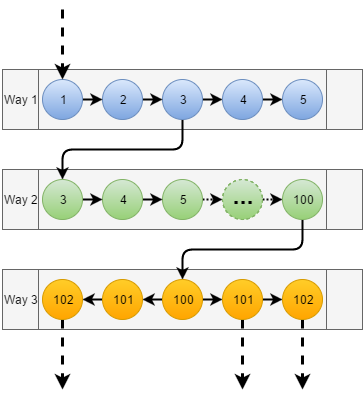
\includegraphics[keepaspectratio, width=0.49\columnwidth]{Images/Way_expansion-order_All}}
	\hfill
	\subfigure[Expanding only the Tower Nodes]{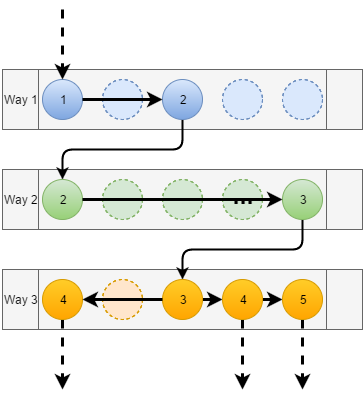
\includegraphics[keepaspectratio, width=0.49\columnwidth]{Images/Way_expansion-order_Tower-Node}}
	
	\caption[Order of Node-expansion]{This illustration shows the order in which Nodes may be expanded inside a Way, and the number of steps required to get from one Way to another. Every Node points to the Node adjacent to it, and so on. Note how Nodes are expanded starting from the entry-point into the Way, which is not always the first Node in the list, and that Nodes may be expanded going in either direction. The abstraction seen in (b) is very similar to how many other hierarchical path-finding systems abstract their data into entry- and exit-points only, and thus reduce the number of steps required to go from one area (or Way) to another; Notice that a constant number of steps are taken in \textit{Way 2} in (b), no matter how many Pillar Nodes the Way contains, but that an additional step has to be taken in \textit{Way 3} because there is a Tower Node between the Nodes in steps 3 and 5.}
	\label{fig:nodeExpansion}
\end{figure}

\begin{figure}
	\centering
	\subfigure[Individual Ways]{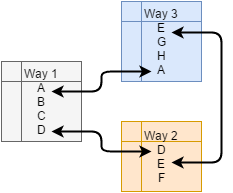
\includegraphics[width=0.49\textwidth]{Images/Connections_Way}}
%	~ %add desired spacing between images, e. g. ~, \quad, \qquad, \hfill etc. 
	%(or a blank line to force the subfigure onto a new line)
	\subfigure[Graph]{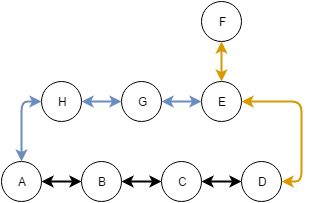
\includegraphics[width=0.49\textwidth]{Images/Connections_Way2}}

	\caption[Connections between Ways]{These images show how Ways may be connected by their Nodes. Note that a connection does not have to originate from the first or last Node in the list.}
	\label{fig:connectionsWays}
\end{figure}

\begin{figure}
	\centering
	\caption[Red path through areas]{This image shows how the route is drawn as a thin red line whenever it passes through a larger area like a building or parking-lot. These red lines are meant to indicate that the actual path through the area is unknown, may be longer than shown on the map, and cannot be guaranteed to be accessible throughout; only the entry- and exit-points are guaranteed to be accessible.}
	\label{fig:areaPath}
	\frame{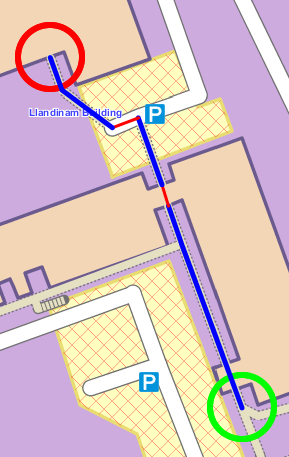
\includegraphics[keepaspectratio, width=0.5\columnwidth]{Images/AStar_Through_building}}
\end{figure}



\section{Programming}
\textbf{NOTES: - DELETE THIS -}
\begin{itemize}
	\item Only really know Java. Java used on many devices \& Mapsforge is written in Java - try to spin this to make it sound positive.
	\item Tried to achieve loose coupling. Everything written in separate modules; changes in one module should not break another. Error/exception handling.
	\item Heavily commented + JavaDoc.
	\item Hash map/table: O(1) time-complexity as opposed to O(n) in Arrays (with unknown index), or O(log n) in binary. Could not make it work. Needs good hash-function, or O( ) might become horrible. O(2n)? memory vs O(n) in both Array and binary? (Reference to cheat-sheet?)
	\item Heap: Maximally efficient Priority Queue - O(log n) vs O(nk). This may be a quote; careful. O(nk) refers to BSc sort?
	\item Empty String: 40 Bytes. Reference/Pointer: 32/64 bit. Cache-miss?
	\item PQ did not reorder when the value of its contents changed - resulted in a big bug.
	\item PQ and expansion list retained Nodes between runs - resulted in sub-optimal path, but faster runtime. (Mention the importance of path re-use).
\end{itemize}

This system has been written in Java, as this is the language most familiar to the author. Many other route-planning applications and map-services have also been developed in Java, so there were plenty of useful examples, discussions, and libraries available on the web.
The IDE used to developed the system is Eclipse\cite{Eclipse_License}. Eclipse has great debugging, auto-complete, and library-import tools, making it very useful in this project -- especially with regard to testing and debugging.

The classes and methods in the system are heavily commented, which should make it easier to follow the execution-flow of the program while debugging. Javadoc has been generated for every class and method (with a few exceptions), as this makes it much easier to use the auto-complete functions provided by Eclipse, but also because this can act as its own sort of system-documentation, which is always kept up-to-date.

The classes and methods are loosely coupled for the most part, but complete loose coupling has not been achieved. It should be possible to change the execution of one method or module without breaking another, but just to make sure that all functionality is still intact after a change has been made, a test-class has been written for every class, and error/exception handling ensures that errors do not propagate further into the system.

The data-structure most suited to storing and indexing all of the Nodes and Ways is a Hash map/table. Provided that the hash-function is quite good, a Hash table has a best-case time-complexity of $O(1)$, which means that it is able to retrieve any data in constant time, regardless of how much information it stores. A poor hash-function can result in the far worse time-complexity of $O(n)$, which is the same as a standard Array (with unknown index), but worse than that of a binary search-tree with a complexity of $O(\log n)$. A Hash table's space-complexity (memory requirements) is $O(n)$, which is the same as a standard Array or binary search-tree, meaning that their space-complexities grow linearly to the number of elements stored. \cite{BigOCheatSheet}

Because a Node might be referenced by more than one Way, the Ways store a reference (or pointer) to the memory-addresses of each of its Nodes in the array of Nodes. This makes sure that every Way references the same Node, and that references to non-existing Nodes can be safely discarded. The Nodes could be stored as Strings, but because an empty String takes up 40 bytes of memory, and a reference/pointer only uses 32/64 bit (depending on the operating system), pointers seems like a better choice. There might be an issue with cache-misses when lots of references to Nodes are read whenever a Way is expanded, but by only expanding Tower Nodes we can reduce the impact this has on the system's runtime.

In order to sort the expanded Nodes by their weights (path-cost, distance to goal, etc.), a priority queue had to be implemented for each of the algorithms that were able to consider these weights. The priority queue used in this system was imported from the Java-library: \verb|java.util.PriorityQueue|. This priority queue is based on a Heap, which is a maximally efficient data-structure to use for queues, and has a time-complexity of $O(log n)$ for insertion, and $O(1)$ for retrieval of the head of the queue (best Node).

Priority queues automatically sort elements as they receive them, but this particular implementation does not reorder Nodes if their weights change after they have been added. This was a big problem in this system, as shorter paths to already discovered Nodes were found constantly, and this lack of reordering made searches significantly slower by not pushing good Nodes to the front of the queue.\\
This problem was solved by first removing the rediscovered Nodes from the priority queue, then adding them again to force a reorder; removing and then adding Nodes has a worst-case time-complexity of $O(2n)$ for each Node though, as the entire queue may need to be searched through to find and remove the Node, at which point we might need to go all the way to the back of the queue again if its path-cost didn't improve much.

Reusing routes between runs can be an effective tool to reduce run-times, as a Node expanded into the old route will indicate that the old path presents the shortest possible path starting at that Node. If path-costs are the same going in either direction startNode$\to$goalNode and goalNode$\to$startNode, then a new path just has to be planned starting at the Node that was moved until either the other Node or the previous path is found.

%The design should describe what you expected to do, and might also explain areas that you had to revise after some investigation.

%Typically, for an object-oriented design, the discussion will focus on the choice of objects and classes and the allocation of methods to classes. The use made of reusable components should be described and their source referenced. Particularly important decisions concerning data structures usually affect the architecture of a system and so should be described here.

%How much material you include on detailed design and implementation will depend very much on the nature of the project. It should not be padded out. Think about the significant aspects of your system. For example, describe the design of the user interface if it is a critical aspect of your system, or provide detail about methods and data structures that are not trivial. Do not spend time on long lists of trivial items and repetitive descriptions. If in doubt about what is appropriate, speak to your supervisor.
 
%You should also identify any support tools that you used. You should discuss your choice of implementation tools - programming language, compilers, database management system, program development environment, etc.

%Some example sub-sections may be as follows, but the specific sections are for you to define. 

%\section{Overall Architecture}

%\section{Some detailed design}

%\subsection{Even more detail}

%\section{User Interface}

%\section{Other relevant sections}